%!TEX root = Thesis.tex

\newcommand\Bx{x}
\newcommand\Bm{m}
\def\v{\vm{v}}
\newcommand\vm[1]{\bm{\mathrm{#1}}}
\renewcommand{\v}{{\mbox{a}^i}}
\newcommand{\z}{z_{t}}
\newcommand{\y}{z_{1:t-1}}

\chapter{Our Approach}
\label{cha:our_approach}

\section{Overview} % (fold)
\label{sec:overview}
Unlike the works presented in the related work we are interested in integrating all stages in solving the problem such as perception, mapping model and action planning into one system. We further present an integrated framework for carrying out the task of detecting the parked cars, integrating occupancy information into a model that is suitable for further planning and planning for actions itself, when carrying out a decision of finding an unoccupied parking lot.
We will further describe the different steps that we have taken on this road as well as the connections between them.

\begin{figure}[ht]%
\centering
\subfloat{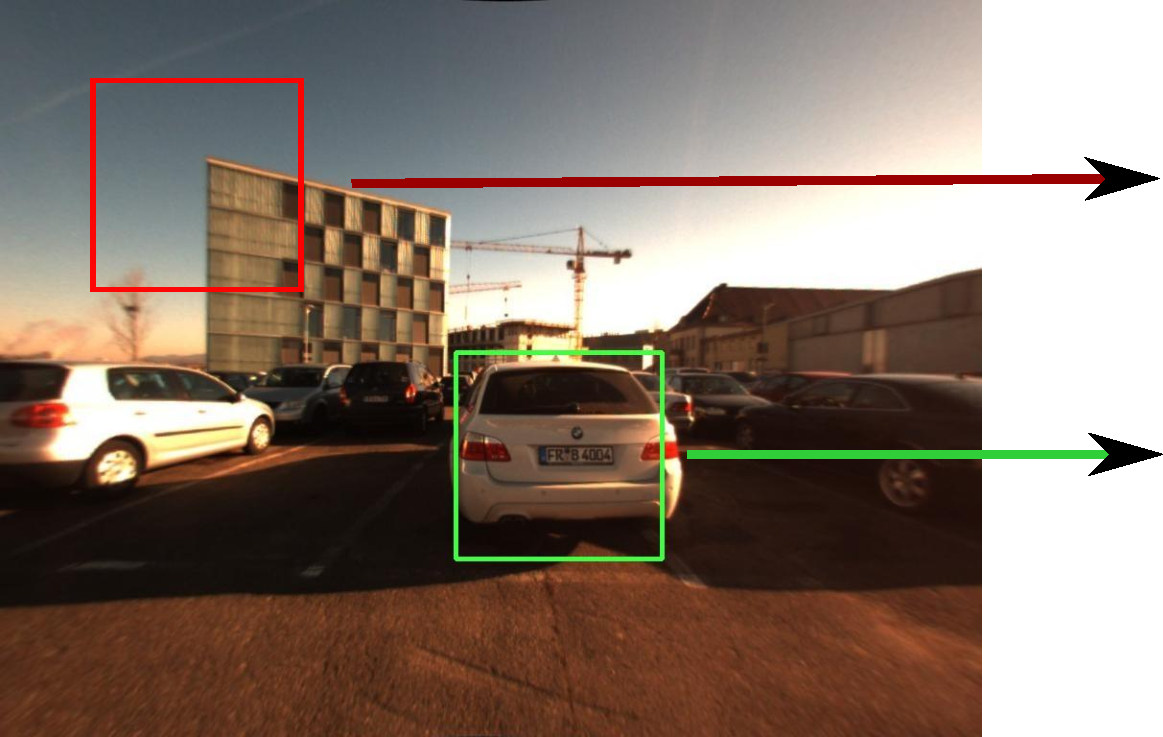
\includegraphics[width=0.6\textwidth]{pictures/detections.pdf}}
\subfloat{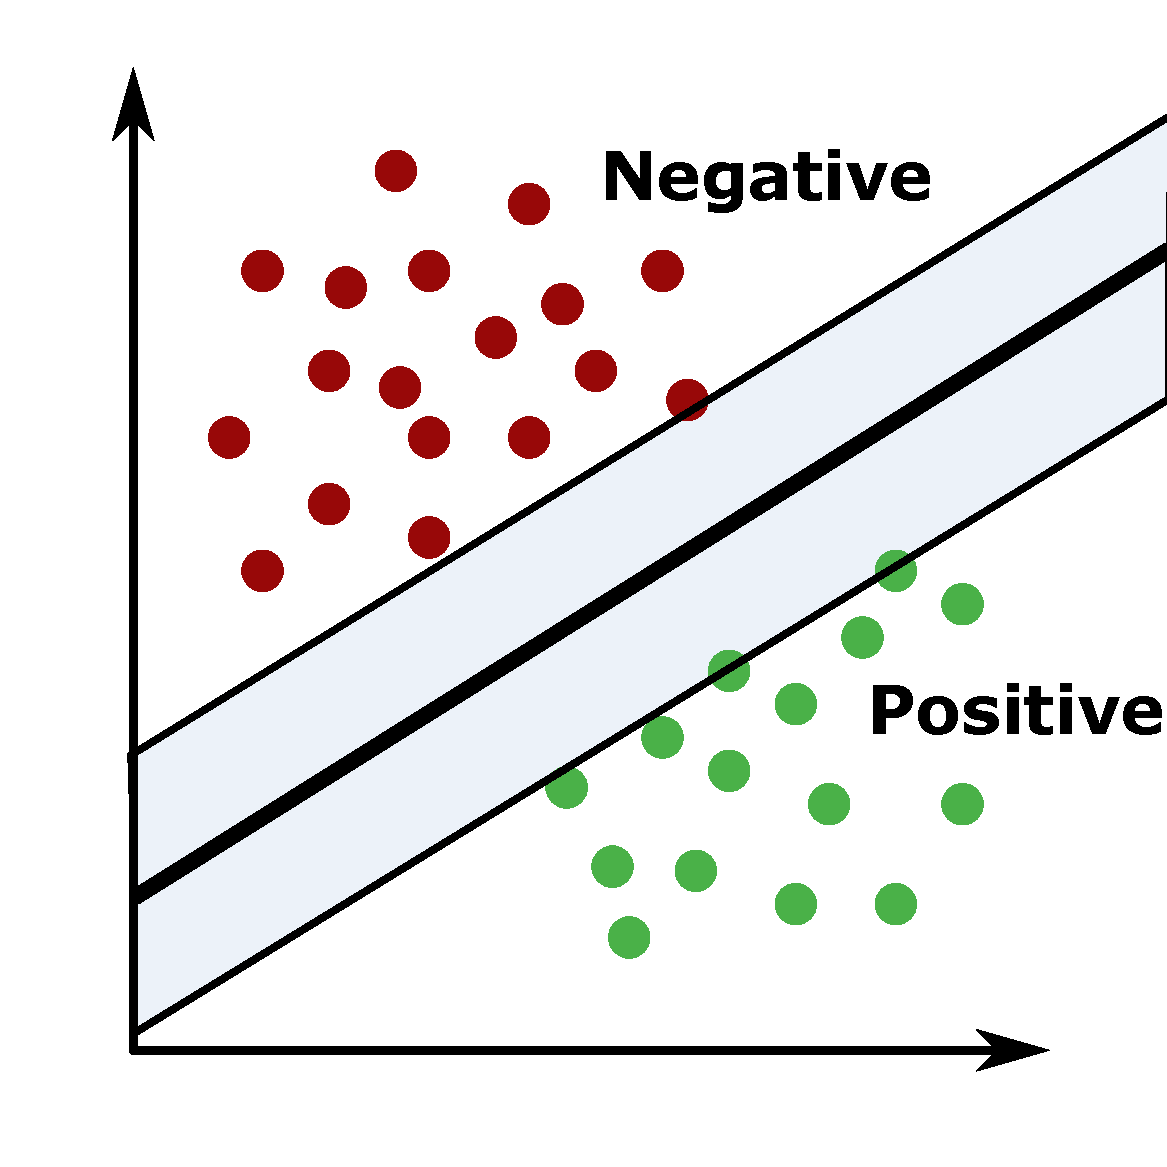
\includegraphics[width=0.4\textwidth]{pictures/svm.pdf}}\\
\subfloat{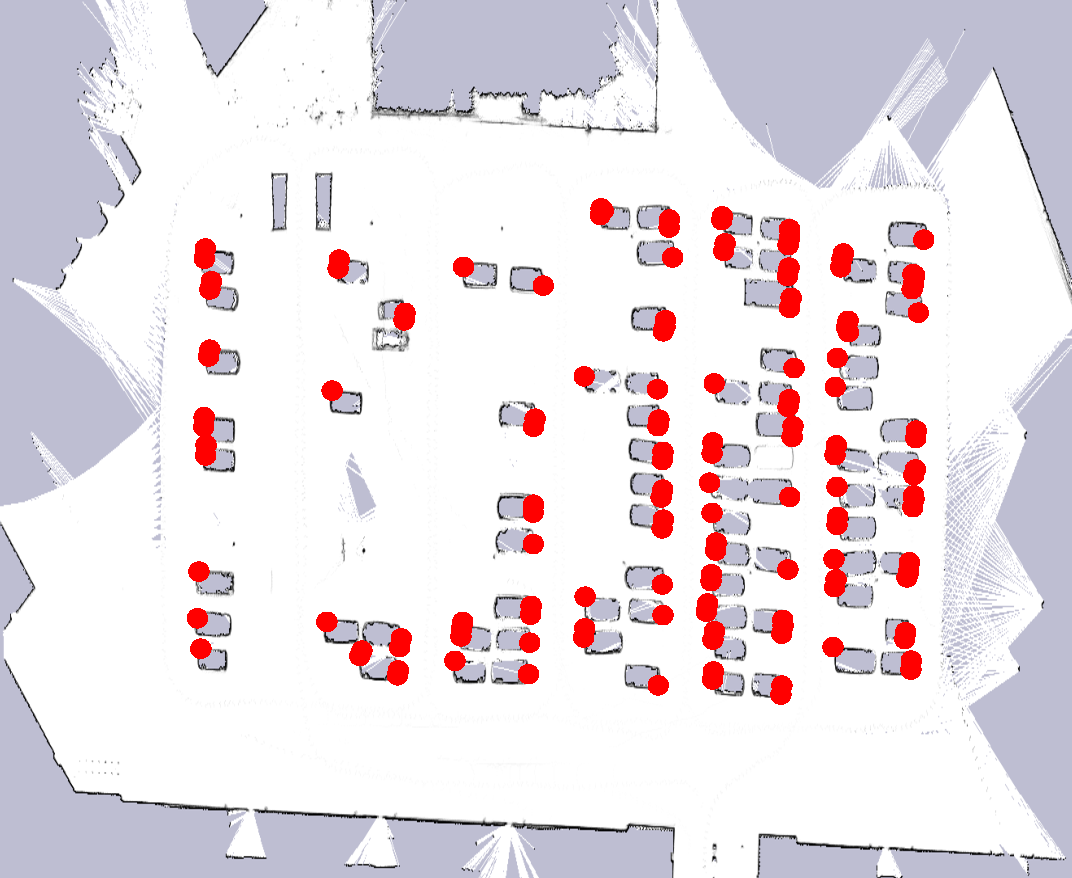
\includegraphics[width=0.6\textwidth]{pictures/laser_fusion.pdf}} \\
\subfloat{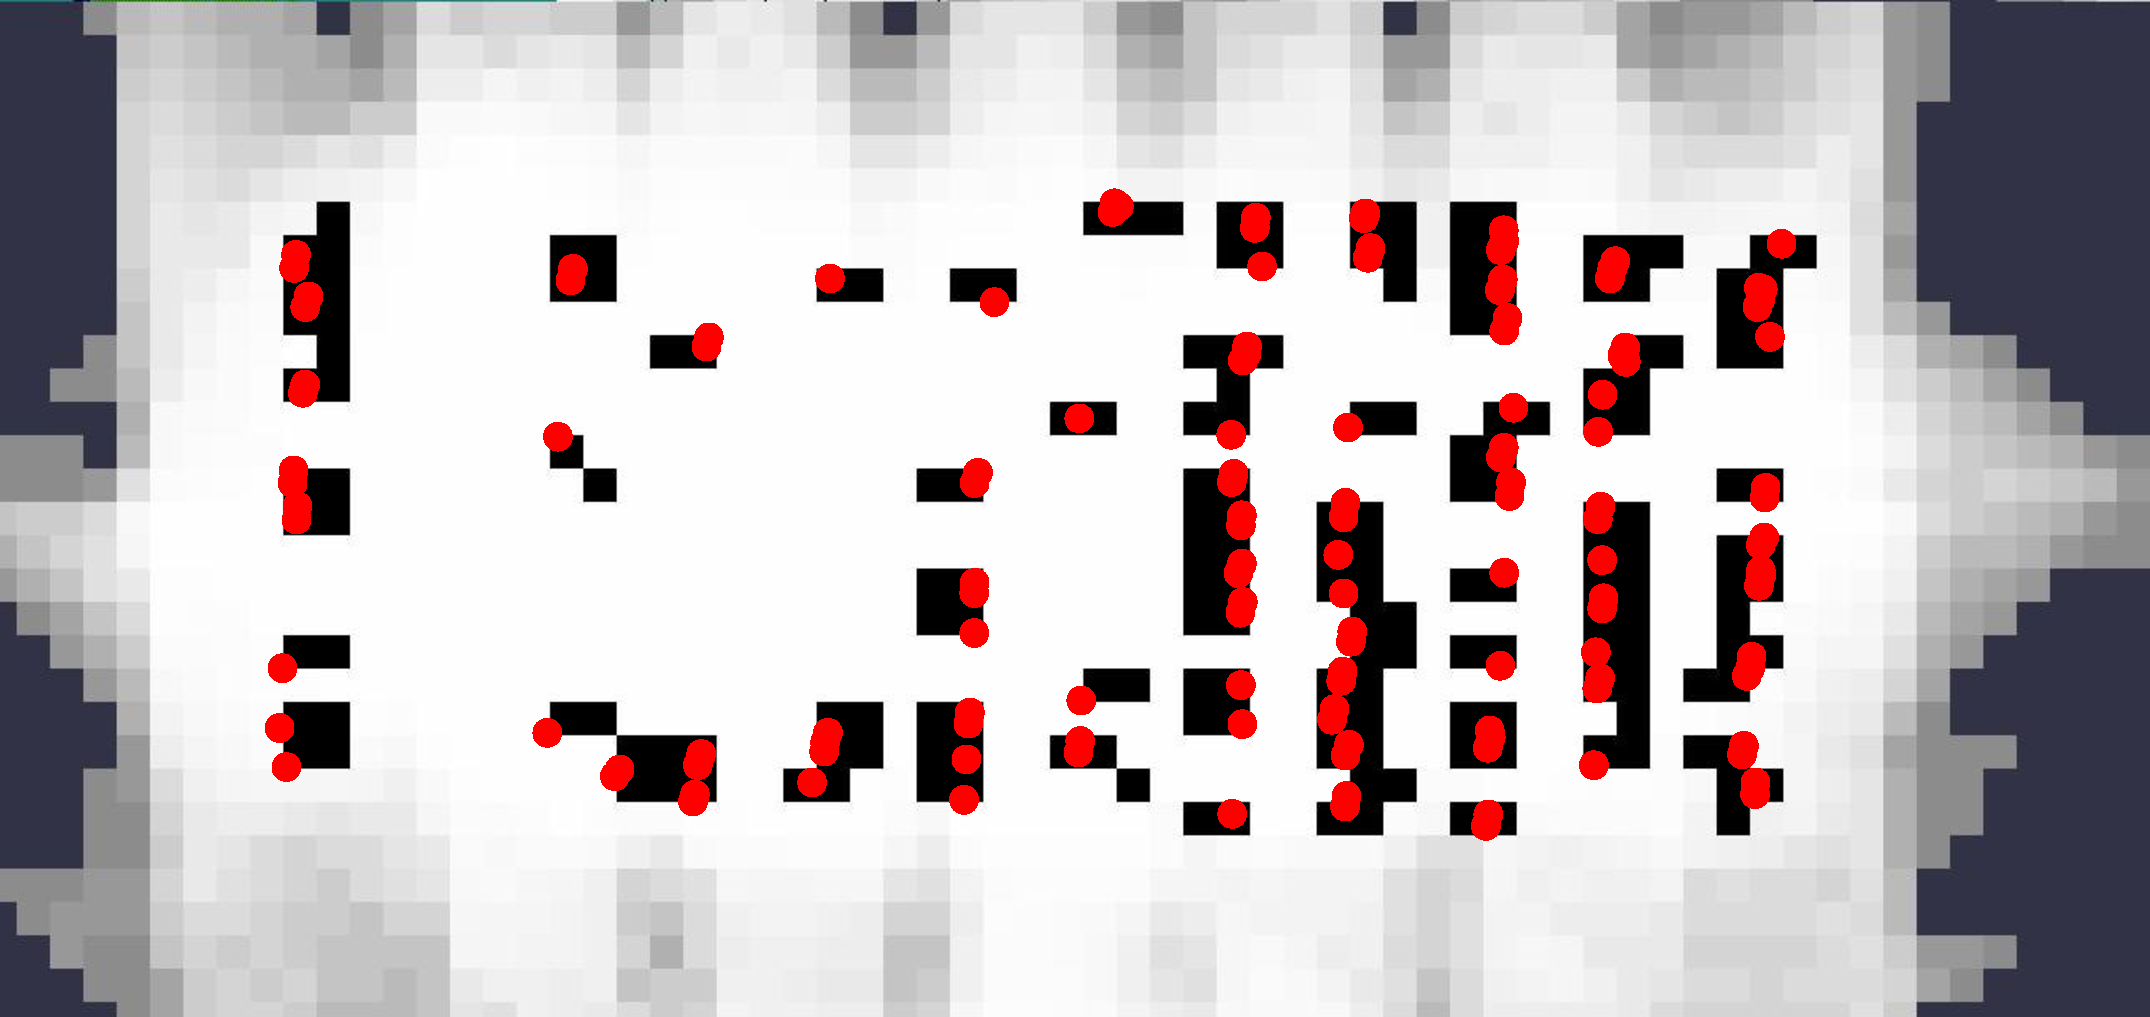
\includegraphics[width=0.6\textwidth]{pictures/occupancy_cars.pdf}} \\
\subfloat{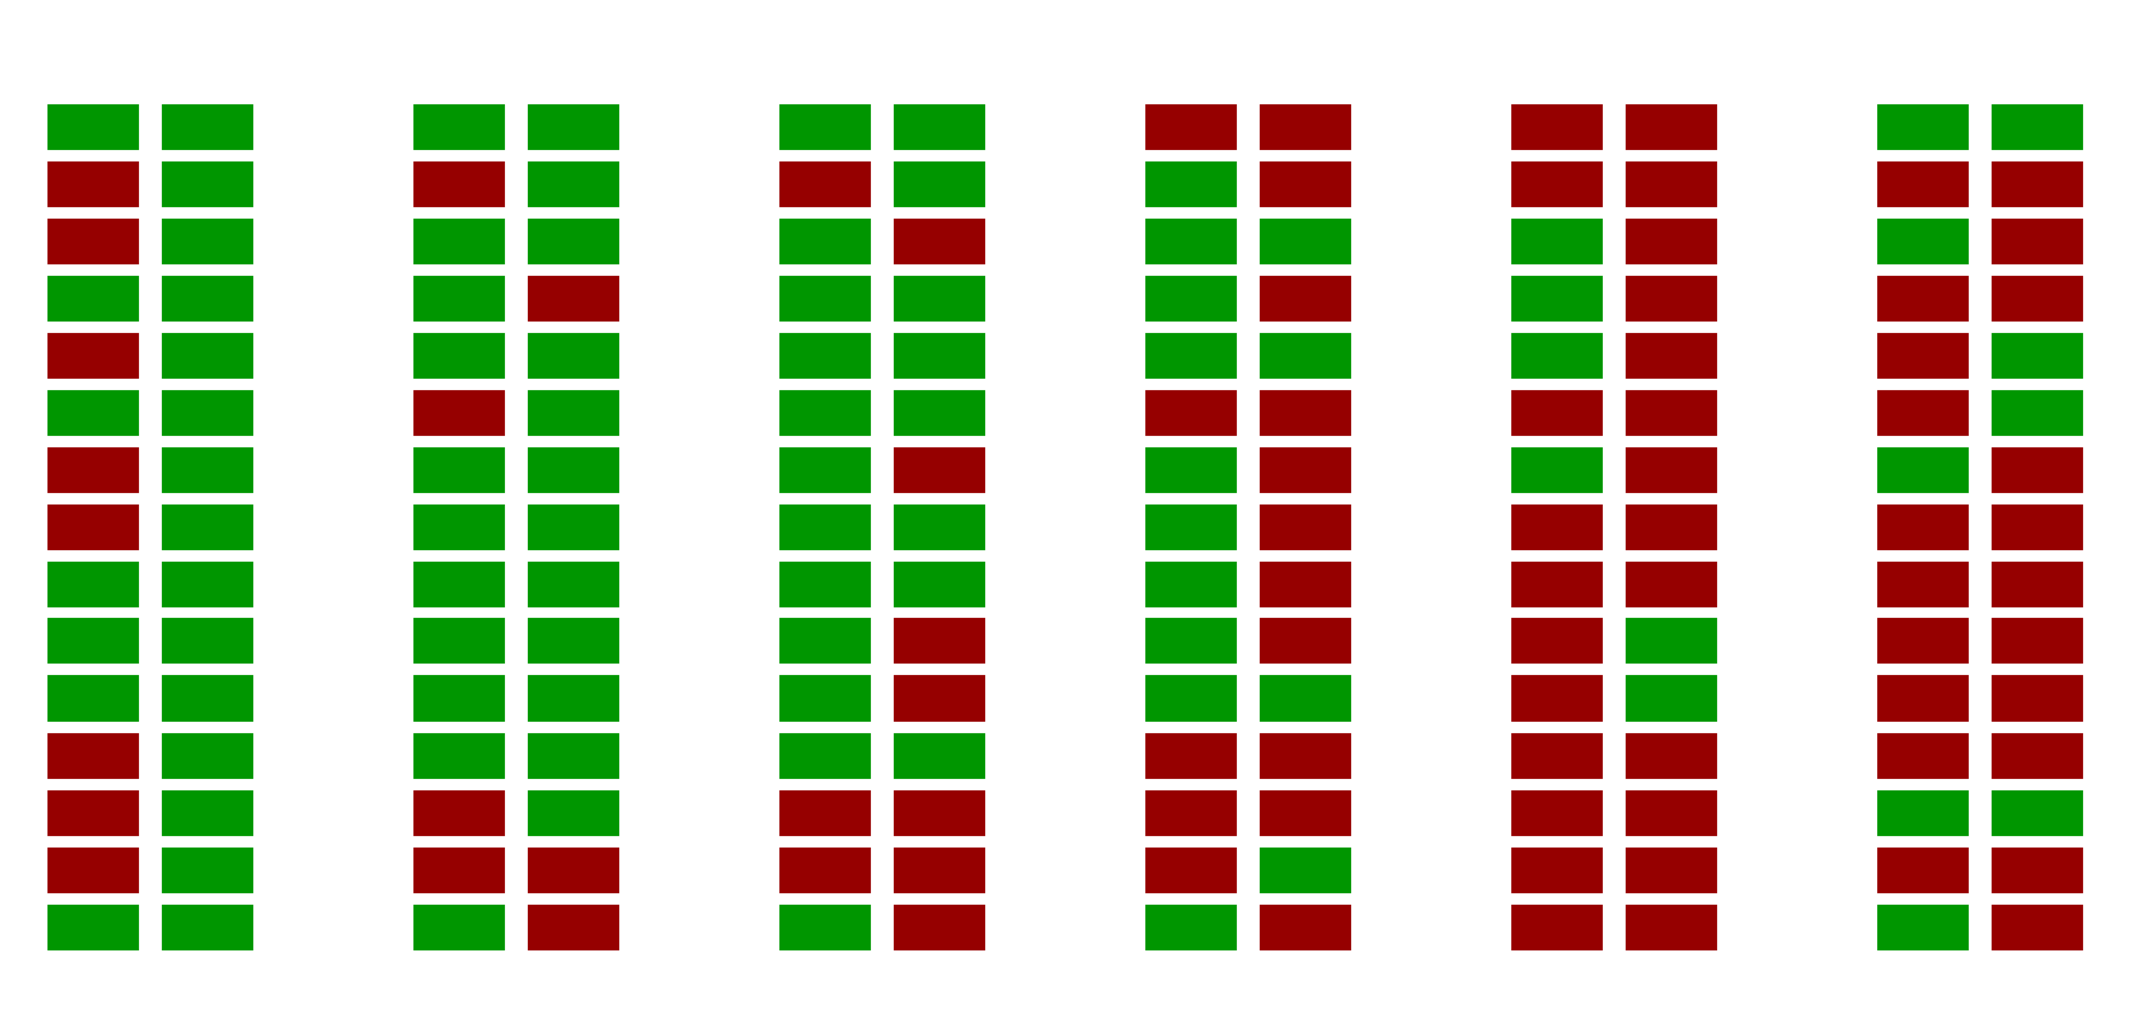
\includegraphics[width=0.6\textwidth]{pictures/parking_lots_detections.pdf}} \\
\caption{Illustration of HOG-based detection and clustering with SVM.}
\label{fig:det_to_svm}
\end{figure}

% section overview (end)

\section{Perception} % (fold)
\label{sec:perception}
    In order to detect the positions of the parked cars we first need to visually recognize the parked cars. To achieve this goal we compared a number of approaches for object detection and classification.

    The work of~\cite{violajones2001} provides good results in the means of
    detection. The main drawback of the proposed method is that it suffers
    from in plane and out of plane rotations and from the illumination
    changes. For the task of car detection it is important to allow for some
    deviations as the cars can differ in shape and angle of detection and it
    may be observed in different lighting conditions. Utilizing the local
    binary patterns (LBPs) as presented by~\cite{lbp2010} solves the
    illumination issues and overall boosts the performance. It is, however,
    alike to Haar features, also vulnerable to rotation and shape changes.
    Also, to the extent of our knowledge, LBP-based method becomes slow on the
    training stage, which is not a problem, but still is an important
    argument, especially on implementation stage.

    Considering the above, we decided to apply the HOG-based detector as
    presented by~\cite{dalal2005}. This method is based on the gradient and it
    therefore deals well with illumination and brightness changes and stays
    robust to the changes in rotation and shape.

    However, whichever algorithm we use, we must make a transition from the
    image space to the world frame. For each detected car we want to know
    precisely where it is situated with relation to the agent's current
    position.

    The relative position of the detected car to the camera, along with the
    global position and orientation of the camera itself, is necessary for
    modeling the occupancy on the global map.

    For this purpose we need to exploit depth information, which we obtain
    from either the range-finder measurements or from the stereo camera.
    We will further focus on each of these options more precisely.

    \subsection{HOG Detector}\label{sub:hog_detector}

    Even though we mostly follow the work of~\cite{dalal2005}, there are still
    differences between our approach and the one presented him. These
    differences are due to the fact that we are interested in detecting cars,
    while the original paper is on detecting people. We are mainly focusing on
    detecting front/rear facing cars, but the approach is easily extended onto
    the side-view as-well. To be able to detect the front and read sides of
    the cars, we need to switch the size of the hog descriptor window from
    $128 \times 64$ pixels to $128 \times 128$ pixels. The idea behind this
    decision is based on generally square-like shape of the cars, when seen
    from front or rear. Therefore, the square drawn around the car will
    contain higher percentage of useful information in comparison to a
    rectangle.

    In the training phase we have considered around 1000 manually chosen $128
    \times 128$ pixel patches containing cars and around 8000 negative
    examples. Each HOG descriptor is then unfolded into a point in a multi-
    dimensional space. These points then have to be clustered into positive
    and negative ones. We describe the background for this decision in the
    next section.

    % subsection hog_classifier (end)

    \subsection{SVM Classifier}\label{sub:svm_classifier}

        In order to carry out the decision in the test data, we train a linear
        SVM classifier on top of all HOG descriptors. A more complex decision
        boundary could of course also be used, but linear SVM, despite its
        simplicity, provides reasonable results as can be seen in
        Section~\ref{cha:experimental_results}.

        SVM is a well known and arguably the most popular algorithm in binary
        clustering, therefore many implementation are readily available. In
        this work we make extensive use of libSVM by~\cite{libSVM2011}.

        The test data detection is carried out in a cascade fashion as
        presented by~\cite{violajones2001} via the sliding window approach.
        For each sliding window content we create a HOG descriptor which is
        then tested against the pre-trained SVM classifier in order to find
        out on which side of the decision boundary it is. If the current HOG
        belongs to the area where cars are then the current sliding window is
        a region of interest and contains a car. Each detection is then stored
        as a rectangle in the coordinates of the image it belongs to. This
        ends the visual detection part and allows us to move on to the 3D
        world.

% subsection svm_classifier (end)

    \subsection{Depth Information}\label{sub:depth_information}

        In this section we will describe in details how the depth information
        was acquired and combined with the visual detections.

        \subsubsection{Stereo Camera}\label{ssub:stereo_camera}

            In order to find the depth from the stereo camera, we need to
            first calculate the disparity image from left and right images
            taken from the video stream. Knowing the internal camera
            parameters we can then reconstruct the relative position of each
            pixel of the disparity image. We first find the distance along the
            camera $Z$ axis: $Z = \frac{fB}{d}$, where $f$ is the focal length
            of the camera, $B$ is the baseline and $d$ is the disparity. After
            $Z$ is determined we can focus on finding $X$ and $Y$ coordinates
            from the ordinary projection equations:

            \begin{eqnarray}
            X = \frac{uZ}{f}
            Y = \frac{vZ}{f}
            \end{eqnarray}

            where $u$ and $v$ are the pixel location in the $2D$ image, $X, Y,
            Z$ is the $3D$ position in the camera frame. When we have the $3D$
            positions for every pixel in the images, we can combine this
            information with the visual detection part. From the previous part
            we have a region of interest in the image coordinates, which
            allows us to accumulate the depth of all pixels that fall into it.
            We can then analyze all of these values to find the distance to
            the car, that is contained in this particular region of interest.
            We considered taking either the mean or the median of the chosen
            values. Given, that the depth that comes from the stereo camera is
            quite noisy and that the depth values of the pixels originate on
            the surface of the car and therefore contain quite a big amount of
            variance, we picked a median as an option as it is the most
            resistant statistic, having a breakdown point of 50$\%$: so long
            as no more than half the data is contaminated, the median will not
            give an arbitrarily large result.

        % sub-subsection stereo_camera (end)
        \subsubsection{Laser Range Finder}\label{ssub:laser_range_finder}

            Even though the stereo camera setup is a lot cheaper and easier to
            mount, it lacks robustness due to the noise that is present in
            disparity images and to some degree to the erroneous values that
            fall into the detected region of interest (such as around the car
            or in the glass parts of it). We therefore also tested a setup
            with a laser range finder. We used a EUROPA robot Obelix which has
            a $270^\circ$ laser mounted approximately on the human knee level.
            This setup proves to be a lot more robust in terms of finding the
            exact $3D$ information about the position of the detected car.
            However, when using laser we need a different approach because
            there we only have images from a monocular camera and thus do not
            have a per-pixel association with the depth field the way we have
            it using the stereo camera. As the laser mounted on the robot
            provides us with $270^\circ$ span it is able to cover
            approximately all the space related to the image from the camera.
            We then need to find the beams, that span through the area covered
            by the image. Given the fact, that the camera is mounted on the
            same $Z$ axis as the laser this can be done in a straightforward
            fashion. We are interested in the beams, the numbers of which
            follows this law:

            \begin{equation}
                 \{ beam_n | \forall n : \gamma_{start} < \alpha_{camera} + \alpha_{0} + \alpha_{n} < \gamma_{end} \}
            \end{equation}

            where $\alpha_{camera}$ is the angle of the camera with respect to
            the direction of the laser, $\gamma_{start}$ and $\gamma_{end}$
            are the starting and ending angle of the detection bounding box in
            the image, $\alpha_{n}$ is the angle of the $n$-th beam in the
            laser frame. All the beam endpoints along with the direction of
            the beams provide us with consistent $3D$ information. In order to
            account for possible occlusions or mistakes we take the median of
            these values as a true position of the detected car. After finding
            the correct car position we move on to the next part and aggregate
            occupancy information into a consistent spacio-temporal map.

        % sub-subsection laser_range_finder (end)
    % subsection depth_information (end)
% section perception (end)

\section{Model} % (fold)
\label{sec:model}

    In the previous sections we have shown the steps of visual detection of
    the cars and finding their real $3D$ world position. Whichever path we
    take in the previous step, now we have a number of real world coordinates,
    that need to be integrated into a consistent map. In this section we will
    present two approaches that we have chosen to target this task.

    \subsection{Occupancy Grids}\label{sub:occupancy_grids}

        In order to map the parking lots along with the occupancy information
        we utilize grid maps (see \nameref{cha:background}:
        \nameref{sec:occupancy_grids}). In this case we model each cell's
        occupancy as a static state Bayes filter.

        Let $P(\v)$ be an occupancy probability estimate of a cell $i$ in the
        environment. Considering the probabilistic nature of occupancy of
        every distinct cell we integrate multiple measurement, taken in
        different times into one model. Following the work
        of~\cite{occupancy_grids}, we obtain an update rule for $P(a_t\mid
        z_{1:t})$. First, we apply Bayes' rule and obtain

        \begin{equation}
        P(a_t \mid  z_{1:t} ) = \frac{P(z_t \mid a_t, \y) P(a_t \mid \y)}{P(z_t \mid \y)}.
        \end{equation}
        \noindent
        We then compute the ratio
        \begin{equation}
        \frac{P(\v\mid z_{1:t})}{P(\neg\v \mid z_{1:t})}
        =
        \frac{P(\z \mid \v, \y)}{P(\z \mid \neg\v, \y)}   \frac{P(\v\mid \y)}{ P(\neg\v\mid \y)}.
        \end{equation}
        \noindent
        Similarly, we obtain
        \begin{equation}
        \nonumber
        \frac{P(\v\mid \z)}{P(\neg\v \mid \z)} = \frac{P(\z \mid \v)}{P(\z \mid \neg\v)}   \frac{P(\v)}{ P(\neg\v)},
        \end{equation}
        \noindent
        which can be transformed to
        \begin{equation}
        \frac{P(\z \mid \v)}{P(\z \mid \neg\v)}
        =
        \frac{P(\v \mid \z)}{P(\neg\v \mid \z)}   \frac{P(\neg\v)}{ P(\v)}.
        \end{equation}
        \noindent
        Applying the Markov assumption that the current observation is
        independent of previous observations given we know that a patch
        contains a parked vehicle gives
        \begin{equation}
        P(\z \mid \v, \y) = P(\z \mid \v),
        \end{equation}
        \noindent
        and utilizing the fact that $P(\neg \v) = 1 - P(\v)$, we obtain
        \begin{eqnarray}
        \lefteqn{\frac{ P(\v \mid z_{1:t}) }{ 1 - P(\v \mid z_{1:t})} = } \nonumber \\
        &&\frac{ P( \v \mid \z)}{ 1 - P(\v \mid \z)}   \frac{ P(\v \mid \y)}{ 1 - P(\v \mid  \y)}   \frac{ 1 - P(\v)}{ P(\v)}.
        \end{eqnarray}

        \noindent
        This equation can be transformed into the following update formula:
        \begin{eqnarray}
        \label{eq:rec_update}
        \hspace{-6mm}\lefteqn{P(\v\mid z_{1:t})=} \nonumber \\
        && \hspace{-10mm} \left[ 1 + \frac{1 - P(\v\mid \z)}{P(\v \mid \z)}
           \frac{1 - P(\v \mid \y)}{P(\v \mid \y)}   \frac{P(\v)}{1 - P(\v)}  \right]^{-1}
        \end{eqnarray}
        \noindent

        In order to gain efficiency, one can furthermore use the log-odds
        formulation of~\cite{moravec1988}, so that the operations
        in~\eqref{eq:rec_update} are realized via addition and subtractions in
        the log-odds space. We can therefore model the probability of each
        cell to be occupied by a parked vehicle at each time $t$. This
        information can be accumulated at any needed time as well as on
        different days. In order to fully define the equation given above, we
        need to define the observation model $P(\v \mid z)$

        \begin{equation}
        \label{eq:observation_model}
            P(a^i | z_t) = \begin{cases} 0.45, & \mbox{if } \mbox{ before detection} \\ 0.9, & \mbox{if } \mbox{ cell stores detection} \\ \mbox{prior}, & \mbox{if } \mbox{ after detection} \end{cases}
        \end{equation}
        Furthermore, the observation model is defined along the rays, that span from the camera position to the defined $z_{\max}$ and along the defined for the camera field of view. Of course, we have an occupancy grid based world, so there has to be a way to compute the cells that fall into the field of view. In order to carry out this action, we first compute left and right further points. We find the cells that form the end frontier by using the Bresenham algorithm as defined by~\cite{bresenham1965}.
        \begin{wrapfigure}{r}{0.4\textwidth}
            \begin{center}
                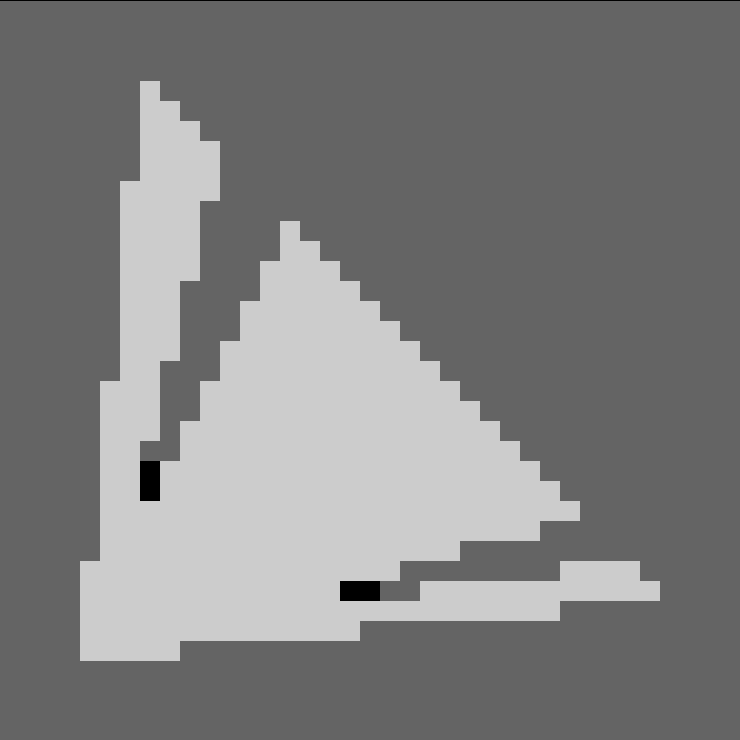
\includegraphics[width=0.35\textwidth]{pictures/testmap.png}
            \end{center}
            \vspace{-20pt}
            \caption{An example of Bresenham based update from a single image with two detected cars.}
            \vspace{-30pt}
            \label{fig:maptest}
        \end{wrapfigure}

        Then, for each cell we carry out the same algorithm from camera cell
        to this query cell. Whenever we encounter a cell, where a car is
        situated, the next cell is also updated as occupied, while all the
        ones that come afterwards are not updated as ``not visible''. This can
        be seen in a small example in Figure~\ref{fig:maptest}. This gives us
        the means of formulating full occupancy grid that can store occupancy
        information from different days. It is theoretically then possible to
        move on to planning.

    % subsection occupancy_grids (end)
    \subsection{Static State Binary Filter in Pre-defined Positions}\label{sub:static_state_binary_filter_in_pre_defined_positions}

        However, occupancy grids have their drawbacks. One of them, especially
        for our setup, is the discretization error. Whenever there are
        multiple detections of the same car from different angles it can
        happen, that the detection is assigned to different cells of the
        occupancy grids. This leads us to the problems of data association and
        therefore difficulties in creating a meaningful accumulated map. This,
        in its turn, leads to wrong decisions of occupancy and ruins or at
        least makes it harder for a planner to carry out a correct decision.
        For now we decided to use a pre-defined set of parking lots, that can
        be set from on-ground data or from aerial images (such as Google
        Maps). The rest of the theory stays untouched. We still make use of
        the static state binary Bayes filter as defined
        in~\eqref{eq:rec_update}. However, the observation model has changed
        to to the absence of the occupancy grid. We now have different
        distinct parking lots, that are represented by a point in the space
        with its coordinates. When we get an observation of occupancy during
        one full session of measurements, we pick the point to update by using
        the closest neighbor from the number of available parking lots. The
        chosen parking lot is updated in a similar way to the occupied case
        of~\ref{eq:observation_model}. After the full session of observation
        is carried out, the untouched cells are updated as free. Though this
        approach does not provide us with a consistent map of the environment
        we still capture the occupancy information of the correctly situated
        in space parking lots, which allows us to form a graph that represents
        the environment and move on to the next
        part:~\nameref{sec:action_planning}.

    % subsection static_state_binary_filter_in_pre_defin (end)
% section model (end)

\section{Action Planning} % (fold)
\label{sec:action_planning}

    Once we have defined the model for mapping, we are able to formally define
    the action planning framework that can lead to an optimal decision in the
    means of picking a path on our way to the parking lot. It depends on the
    application what an optimal decision is. Whenever we try to find a parking
    space it is usually the case, that there are parts of the parking lot
    which are better suited for parking. Usually it means, that these parts
    are closer to the destination where all the people lean to. This also
    means that the ``better'' parts of the parking lots are more occupied than
    the other, which leads us to a trade-off between going straight to the
    closest, but likely occupied parking lot, which results in spending time
    searching for a new one or parking in a more distant area, most likely
    free, but it takes a while to walk from there to the goal. Given the
    constraints described above, the framework that we present focuses on
    finding the solution that minimizes the expected time spent on finding a
    free parking spot and walking from the found one to the goal.

    As stated in the work of~\cite{tipaldiICRA11}, MDPs can be used when there is a need to maximize the joint rewards instead of greedily going for the best possible goal.
    We follow similar approach, while defining rewards and transition probabilities based on the environment that we have in our problem.

    In order to solve the given problem in an optimal way, we define rewards, which depict the time spent for each transition from state to state an agent can take. We then use the Markov Decision Processes as described in section~\ref{sec:markov_descision_processes} to find a path that maximizes the reward.
    The resulting path does not go for the best spot, but maximizes the probability of encountering a free parking lot, while trying keeping the length of the search path as short as possible.

    As it is stated in section~\ref{sec:markov_descision_processes}, we need to define rewards and actions in order to fully define an MDP problem.
    First, lets start, by defining the state space. The states are defined as the vertices of the graph $V$, each of which represents a point in space. The graph also has edges $E$ a function $V \rightarrow V$, that correspond to the actions that can be carried out from one state to another. In the grid based situation, the states are the grids cells. In the case, where we explicitly map the parking lots --- they, along with their spacial information form the vertices of the graph.
    In order to define rewards and probabilities of actions we need to define the set of all actions that can be carried out. We are assuming to be in a world, where only five actions are defined --- ``up'': $\uparrow$,
    ``down'': $\downarrow$, ``left'': $\leftarrow$, ``right'': $\rightarrow$ and ``park''. Formally:
    \begin{eqnarray}
        A_{\mbox{move}} = \{ \uparrow, \downarrow, \leftarrow, \rightarrow \} \\
        a_{\mbox{park}} = \mbox{``park''} \\
        A = A_{\mbox{move}} \cup a_{\mbox{park}}
    \end{eqnarray}
    Now we can define the reward function $R(s, s', a)$ as well as transition function $P(s| s', a)$.
    Let us first start with probabilities. For four actions that describe moving around the parking lot in a car we considered the probability of moving from any state to the next one (if possible) to be equal to 1, while the probability of parking in a particular state is equal to the occupancy probability of the state:
    \begin{eqnarray}
        \forall (s, s') \in E, \forall a \in A_{\mbox{move}} : P(s| s', a) = 1 \\
        \forall s \in V, (s,s_{\mbox{goal}}) \in E : P(s| s_{\mbox{goal}}, a_{\mbox{park}}) = P(\mbox{free})
    \end{eqnarray}
    where $P(\mbox{free})$ is a probability of a parking lot to be free, observed through a period of time.
    To be consistent and to fully define the transaction model, we also need to set the remaining probabilities (the ones not set before) to the values such that $\forall s, s' \in V, (s, s') \in E : \sum_{s'}P(s| s', a) = 1$.
    This resolves to staying in the same state when trying to carry out an unavailable or improbable action in any state. \\
    For example: it is clear, that staying in the left most corner of the parking lot and carrying an action to go left, should result in staying in the same spot and while carrying out an action of parking, with the probability of $0.6$ has a $0.4$ chance to stay in the same place.

    Another part of defining the MDP is the definition of the reward function
    $R(s,s',a)$. The motivation behind the rewards is based on the time it
    takes an agent to carry out an action. For now we assume, that it takes us
    a constant time for moving from one state $s$ to another $s'$. If we
    cannot carry out the action and are forced to stay in the same position,
    we anyway lose the time. This describes the fact that each action takes
    time. We therefore define a negative reward for carrying out any movement:

    \begin{equation}
        \forall (s, s') \in E, \forall a \in A_{\mbox{move}}: R(s, s', a) = R(s, s, a) = \mbox{-const}
    \end{equation}

    We have defined the costs of moving, which ``tells'' our agent, that the best strategy would be to stay in one place. However, this is not the behavior we expect from an intelligent agent, so we need to define the rewards of reaching the goal state. The rewards should still be time based, but they have to form a decreasing linear function as the state closer to the destination should get a bigger reward than the one that is situated further. We decided to set the reward to $r_{\max} - r_s$, where $r_s = \sqrt{(s - s_{\mbox{goal}}) {(s - s_{\mbox{goal}})}^T}$ is a distance between the arbitrary state $s \in \mathbb{R}^2$ and $r_{\max} = \max_{s \in V}r_s$ is the greatest of those distances. Therefore:
    \begin{equation}
        \forall s \in V, (s,\mbox{goal}) \in E : R(s, s_{\mbox{goal}}, a_{\mbox{park}}) = r_{\max} - r_s
    \end{equation}
    This guarantees, that the agent will try to find the way to maximize the reward he gets from parking in the described locations.
    Combining the defined transition model and the reward function allows us to fully define the MDP, which we are then able to solve with the policy iteration method as described in section \nameref{sec:markov_descision_processes}. The solution to the MDP guarantees to find an optimal solution to the given problem, which, given the nature of our reward functions is also an optimal solution from the human point of view.

    However, the MDPs can sometimes fail on the given problem. The failure can be described as follows: the agent carries out an optimal strategy up to the point when he needs to carry out the parking decision. Let us imagine for a moment that the parking lot at which the agent wants to park is occupied. From the point of view of the MDPs the optimal decision would be to wait and try once again, which is clearly a suboptimal decision. Therefore, we also need to plug in the observations of the world. Whenever we move past some parking lot we check if it is occupied and update the occupancy probability in this state to 1 or 0 respectively. We are then able to carry out a decision having a better background. To find what the next optimal action would be, we start the policy iteration on the newly defined graph for MDPs, providing the last found policy as initial. Under the assumption, that changing the occupancy probability of the observed vertices does not dramatically change the movement strategy of the agent, this yields optimal planning time because the policy iteration algorithm is carried out to the point when the policy does not change.

% section action_planning (end)
